\chapter{Experimental Design}

\section{Materials and Methods}
\subsection{Materials}
The bioprinter’s printing parameters are adjusted using a computer which behaves as an interface and the prints produced in each trial of the experiment are measured using a measuring tape and digital vernier caliper. This experimental setup is shown below in Figure~\ref{fig:experimentalSetup}:
 \begin{figure}[h]
    \centering
    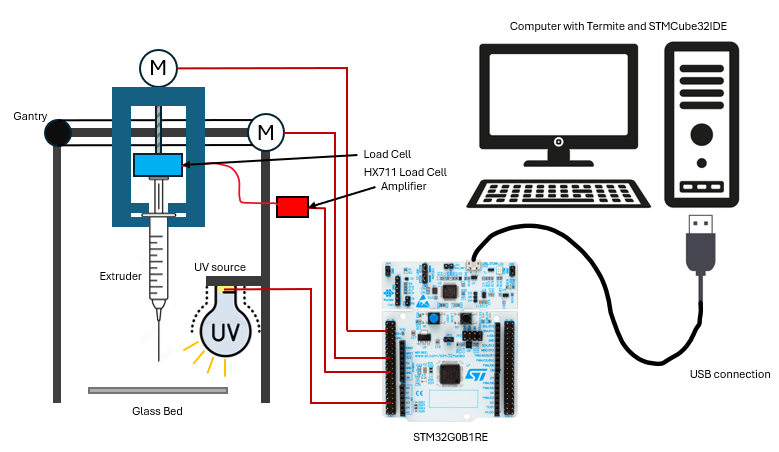
\includegraphics[scale=0.7]{figs/ExperimentalSetup.png}
    \caption{Experimental Setup (please change pic)}
    \label{fig:experimentalSetup}
\end{figure}
\subsection{Equipment Specifications}
\subsubsection*{GelMA Specifications}
\subsubsection*{Bioprinter Specifications}
\subsubsection*{Software}
\subsection{Methods}
\subsubsection*{Experimental Setup Procedure}
\subsubsection*{Test Procedure}
\section{Discussion of Results and Conclusion}